%needs Packages:
% - \usepackage[export]{adjustbox} for  "valign=t"

\section{Wichtige Funktionen}
\begin{tabular}{p{5cm} p{12.5cm}}
  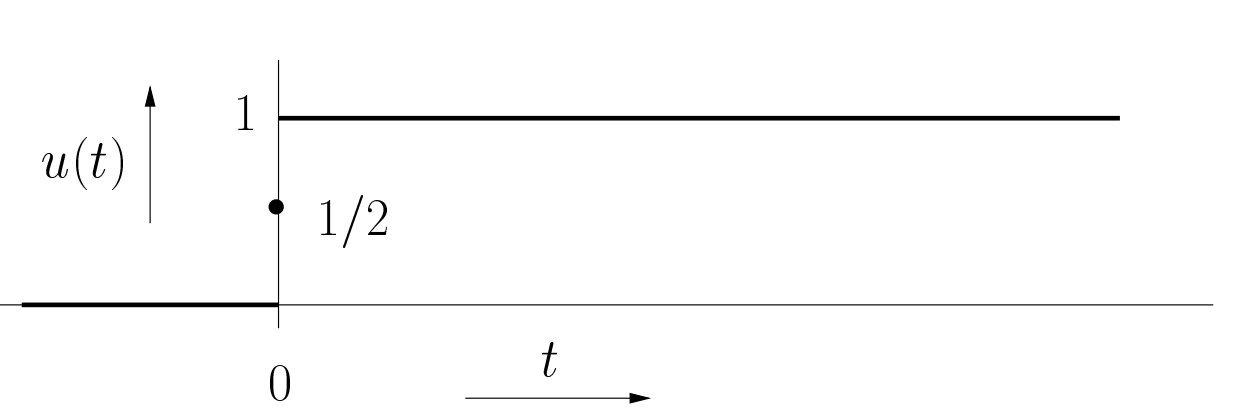
\includegraphics[width = 5cm, valign=t]{include/Wichtige Funktionen/img/Sprungfunktion.png} &
  \textbf{Sprungfunktion (Heaviside)}
  \footnotesize
  Normierter Einschaltvorgang
  $$H(t) = \begin{cases}
               0 \textrm{ für }  t<0,                                                                      \\
               [\frac{1}{2} \textrm{ für }  t = 0,] \textrm{ \tiny(nicht immer vorhanden; dann 1 für t=0)} \\
               1 \textrm{ für }  t >0.
             \end{cases}   $$
  \\
  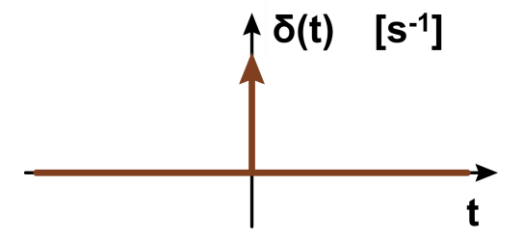
\includegraphics[width = 5cm, valign=t]{include/Wichtige Funktionen/img/Impulsfunktion.png} &
  \textbf{Diracimpuls} \tiny (auch Impuls-/Deltafunktion, Delta-Distribution)
  \footnotesize \newline
  Unendlicher kurzer normierter Impuls mit unendlicher Amplitude
  $$\int\limits _{-\infty} ^{+\infty} f(t) \cdot \delta (t-t_0) dt = f(t_0) \;
    \int\limits _{-\infty} ^{+\infty} f(t) \cdot \delta (t) dt = f(0) \;
    \int\limits _{-\infty} ^{+\infty} \delta (t) dt = 1$$
  TODO: 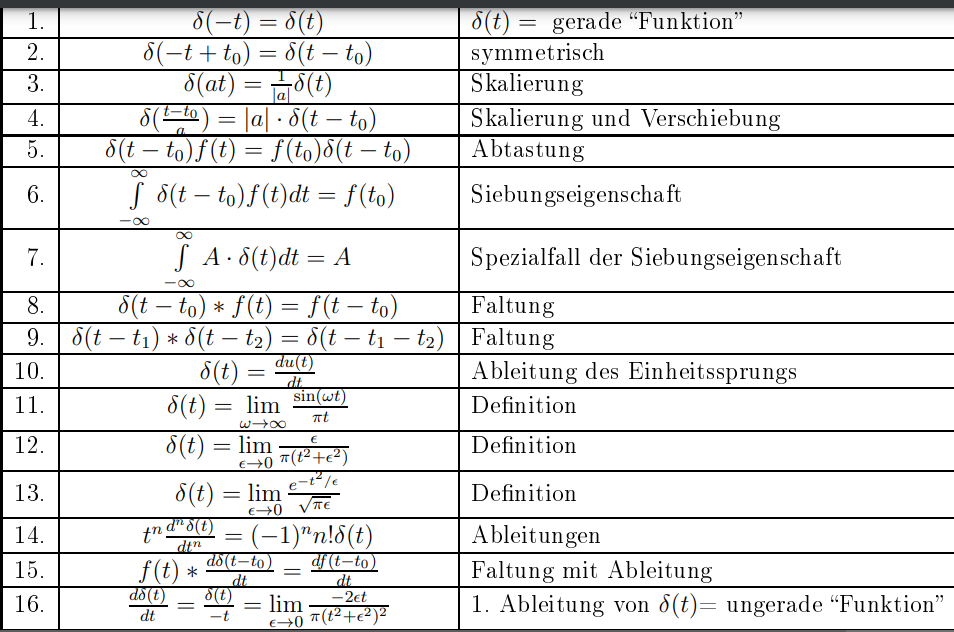
\includegraphics[width=5cm]{include/Wichtige Funktionen/img/Eigenschaften _delta.png}   \\
  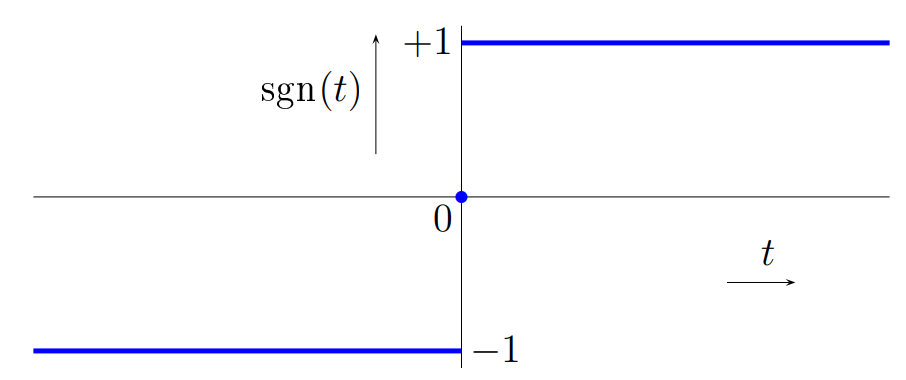
\includegraphics[width = 5cm, valign=t]{include/Wichtige Funktionen/img/Signumfunktion.png} &
  \textbf{Signumfunktion} (Vorzeichenfunktion)
  \footnotesize
  $$sgn(t) = \begin{cases}
                 -1 \textrm{ für }  t<0,  \\
                 0 \textrm{ für }  t = 0, \\
                 1 \textrm{ für }  t >0.
               \end{cases}   $$                                                           \\
  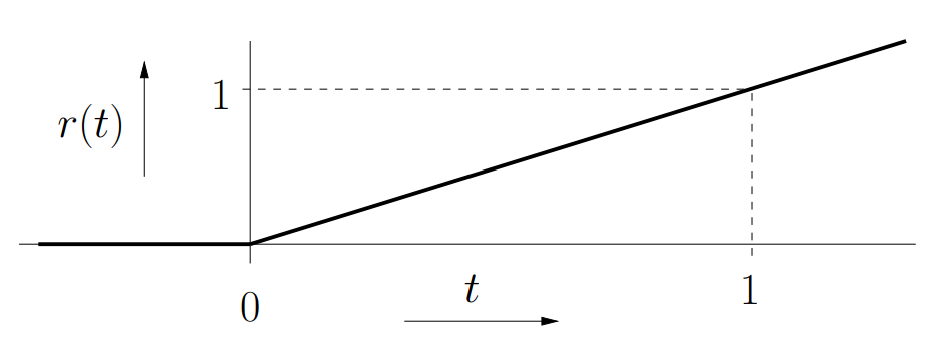
\includegraphics[width=5cm, valign=t]{include/Wichtige Funktionen/img/Rampenfunktion.png}   &
  \textbf{Rampenfunktion}
  \footnotesize
  $$r(t) = \begin{cases}
               0 \textrm{ für } t \leq 0, \\
               t \textrm{ für } t > 0.
             \end{cases}$$                                                           \\
  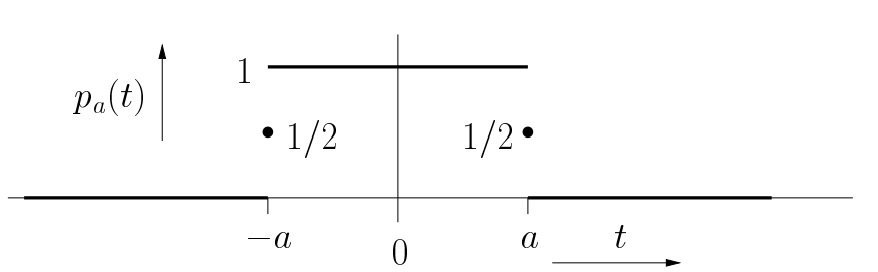
\includegraphics[width=5cm, valign=t]{include/Wichtige Funktionen/img/Rechteckimpuls.png}   &
  \textbf{Rechteckimpuls}
  \footnotesize
  $$p_a(t) = u(t+a)-u(t-a)= \begin{cases}
                                1 \textrm{ für } |t| < a,           \\
                                \frac{1}{2} \textrm{ für } |t| = a, \\
                                0 \textrm{ für } |t| > a.
                              \end{cases} $$                                 \\
  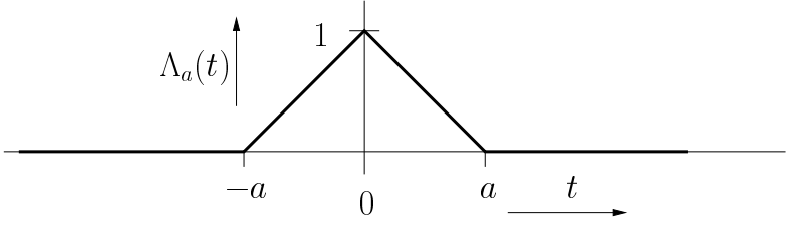
\includegraphics[width=5cm, valign=t]{include/Wichtige Funktionen/img/Dreieckimpuls.png}    &
  \textbf{Dreieckimpuls}
  \footnotesize
  $$\Lambda(t) = \begin{cases}
                     1 - \frac{|t|}{a} \textrm{ für } |t| < a \\
                     0 \textrm{ für } |t| \geq a
                   \end{cases}$$                                       \\
  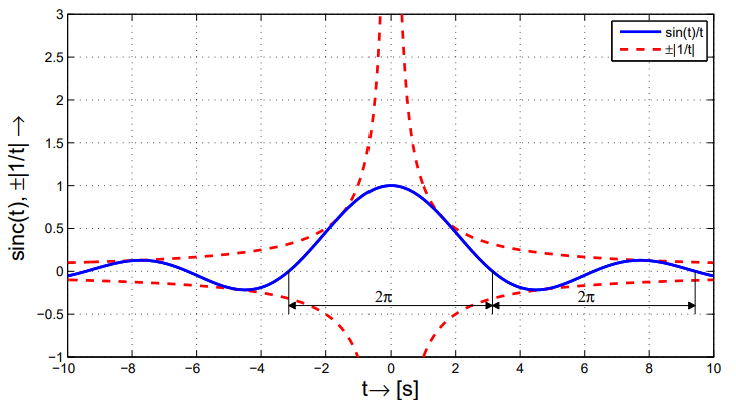
\includegraphics[width=5cm, valign=t]{include/Wichtige Funktionen/img/SincFunktion.png}     &
  \textbf{Sinc-Funktion}
  \footnotesize
  $$sinc(t) = \frac{sin(t)}{t} \forall t$$                                                                                     \\
\end{tabular}
